\documentclass[12pt]{article}
\usepackage[utf8]{inputenc}
\usepackage[T1]{fontenc}
\usepackage[english]{babel}
\usepackage{amsmath, amssymb, amsthm}
\usepackage{geometry}
\usepackage{titling}
\usepackage{fancyhdr}
\usepackage{lipsum}
\usepackage{parskip}
\usepackage{forest}
\usepackage{tikz}
\usepackage{stmaryrd}
\usepackage{listings}
\usepackage{graphicx}
\usepackage{float}
\usepackage{alphalph}
\usepackage{cancel}
\usepackage{textgreek}
\usepackage{titlesec}
\usepackage{enumitem}
\usepackage{dsfont}
\usepackage{caption}
\usepackage{cancel}
\usepackage{rotating}


\geometry{top=4cm, bottom=4cm, left=3.5cm, right=3.5cm}
\pagestyle{fancy}
\fancyhf{}
\rhead{Pierre Pili $\cdot$ Isée Biglietti}
\lhead{Advanced Econometrics}
\cfoot{\thepage}
\setlength{\headheight}{14.49998pt}
\addtolength{\topmargin}{-2.49998pt}

\titleformat{\section}{\small\bfseries}{\thesection}{1em}{}
\renewcommand{\thesubsection}{\arabic{section}.\arabic{subsection}}
\renewcommand{\thesubsubsection}{\arabic{section}.\arabic{subsection}.\alph{subsubsection}}

\title{Robust Replication}
\author{PILI Pierre $\cdot$ BIGLIETTI Isée}
\date{\today}

\titleformat{\subsection}[hang]
  {\normalfont\small\bfseries}
  {\thesubsection}
  {1em}
  {}
\renewcommand{\thesubsection}{\roman{subsection}}
\setlist[enumerate,1]{label=\textbf{\arabic*}.}
  
\begin{document}
\maketitle


% Table created by stargazer v.5.2.3 by Marek Hlavac, Social Policy Institute. E-mail: marek.hlavac at gmail.com
% Date and time: Sam, déc 28, 2024 - 12:35:24
\begin{table}[!htbp] \centering 
  \caption{Robust Descriptive Statistics} 
  \label{} 
\scriptsize 
\begin{tabular}{@{\extracolsep{0pt}} cccccccccc} 
\\[-1.8ex]\hline 
\hline \\[-1.8ex] 
var & median & mean & min & max & sd & iqr & skewness & kurtosis & non\_missing \\ 
\hline \\[-1.8ex] 
gpdistroad & $1$ & $1.50$ & $0$ & $10$ & $2$ & $1.70$ & $2.40$ & $9.30$ & $0.91$ \\ 
totpop & $1,700$ & $2,100$ & $630$ & $13,000$ & $1,500$ & $940$ & $4.70$ & $30$ & $1$ \\ 
lit & $0.35$ & $0.36$ & $0.12$ & $0.66$ & $0.12$ & $0.17$ & $0.38$ & $2.60$ & $1$ \\ 
frsc & $0.21$ & $0.24$ & $0.01$ & $0.74$ & $0.14$ & $0.18$ & $1.10$ & $4.40$ & $1$ \\ 
frobc & $0.48$ & $0.49$ & $0.06$ & $0.94$ & $0.17$ & $0.28$ & $0.17$ & $2.40$ & $1$ \\ 
density & $5.30$ & $6.40$ & $1.30$ & $36$ & $4.40$ & $3.40$ & $3$ & $18$ & $1$ \\ 
scaste & $0$ & $0.15$ & $0$ & $1$ & $0.36$ & $0$ & $2$ & $4.80$ & $0.94$ \\ 
scaste2 & $0$ & $0.43$ & $0$ & $1$ & $0.50$ & $1$ & $0.27$ & $1.10$ & $0.94$ \\ 
sgen & $1$ & $0.52$ & $0$ & $1$ & $0.50$ & $1$ & $$-$0.09$ & $1$ & $0.97$ \\ 
fe2 & $0$ & $0.40$ & $0$ & $1$ & $0.49$ & $1$ & $0.42$ & $1.20$ & $0.91$ \\ 
fe3 & $0$ & $0.27$ & $0$ & $1$ & $0.44$ & $1$ & $1.10$ & $2.10$ & $0.91$ \\ 
me2 & $0$ & $0.09$ & $0$ & $1$ & $0.29$ & $0$ & $2.90$ & $9.20$ & $0.92$ \\ 
me3 & $0$ & $0.15$ & $0$ & $1$ & $0.36$ & $0$ & $2$ & $4.90$ & $0.92$ \\ 
tepupr & $73$ & $86$ & $7.50$ & $320$ & $52$ & $48$ & $2.20$ & $9$ & $1$ \\ 
elec & $1$ & $0.77$ & $0$ & $1$ & $0.42$ & $0$ & $$-$1.30$ & $2.60$ & $0.94$ \\ 
phone & $1$ & $0.66$ & $0$ & $1$ & $0.47$ & $1$ & $$-$0.68$ & $1.50$ & $0.93$ \\ 
index & $3$ & $2.60$ & $0$ & $4$ & $0.98$ & $1$ & $$-$0.27$ & $2.50$ & $0.98$ \\ 
op & $1$ & $0.58$ & $0$ & $1$ & $0.49$ & $1$ & $$-$0.32$ & $1.10$ & $1$ \\ 
dms14 & $0$ & $0.08$ & $0$ & $1$ & $0.27$ & $0$ & $3.10$ & $11$ & $1$ \\ 
dms15 & $0$ & $0.36$ & $0$ & $1$ & $0.48$ & $1$ & $0.58$ & $1.30$ & $1$ \\ 
dms16 & $1$ & $0.82$ & $0$ & $1$ & $0.38$ & $0$ & $$-$1.70$ & $3.80$ & $1$ \\ 
dms19 & $0$ & $0.15$ & $0$ & $1$ & $0.36$ & $0$ & $1.90$ & $4.70$ & $1$ \\ 
dmaq3 & $0$ & $0.04$ & $0$ & $1$ & $0.19$ & $0$ & $5$ & $26$ & $1$ \\ 
dmaq2 & $1$ & $0.93$ & $0$ & $1$ & $0.25$ & $0$ & $$-$3.40$ & $13$ & $1$ \\ 
dmph4 & $0$ & $0.18$ & $0$ & $1$ & $0.38$ & $0$ & $1.70$ & $3.80$ & $1$ \\ 
dmph5 & $0$ & $0.07$ & $0$ & $1$ & $0.26$ & $0$ & $3.30$ & $12$ & $1$ \\ 
dmph6 & $0$ & $0.40$ & $0$ & $1$ & $0.49$ & $1$ & $0.39$ & $1.20$ & $1$ \\ 
dmph7 & $0$ & $0.08$ & $0$ & $1$ & $0.27$ & $0$ & $3.10$ & $11$ & $1$ \\ 
lon & $82$ & $82$ & $79$ & $100$ & $3.60$ & $2.50$ & $4.20$ & $21$ & $1$ \\ 
lat & $26$ & $26$ & $25$ & $29$ & $0.80$ & $1.30$ & $0.48$ & $3$ & $1$ \\ 
alt & $110$ & $110$ & $62$ & $160$ & $26$ & $46$ & $$-$0.09$ & $2.20$ & $1$ \\ 
rain & $1,000$ & $1,100$ & $810$ & $1,900$ & $310$ & $200$ & $1.70$ & $5$ & $1$ \\ 
studentattendance & $0.83$ & $0.72$ & $0$ & $1$ & $0.25$ & $0.50$ & $$-$0.80$ & $2.90$ & $0.96$ \\ 
score & $6$ & $6$ & $0$ & $22$ & $4.80$ & $9$ & $0.26$ & $1.80$ & $0.90$ \\ 
meanscore & $$-$0.13$ & $$-$0.13$ & $$-$1.40$ & $3.20$ & $0.99$ & $1.80$ & $0.26$ & $1.80$ & $0.90$ \\ 
districtid & $13$ & $13$ & $1$ & $26$ & $7.40$ & $13$ & $0.08$ & $1.80$ & $1$ \\ 
block & $13$ & $14$ & $1$ & $26$ & $7.50$ & $13$ & $0.04$ & $1.80$ & $1$ \\ 
grampanchayat & $65$ & $65$ & $1$ & $130$ & $38$ & $66$ & $0.03$ & $1.80$ & $1$ \\ 
\hline \\[-1.8ex] 
\end{tabular} 
\end{table} 

\begin{figure}[p]  % 'p' place la figure sur une page dédiée
    \centering
    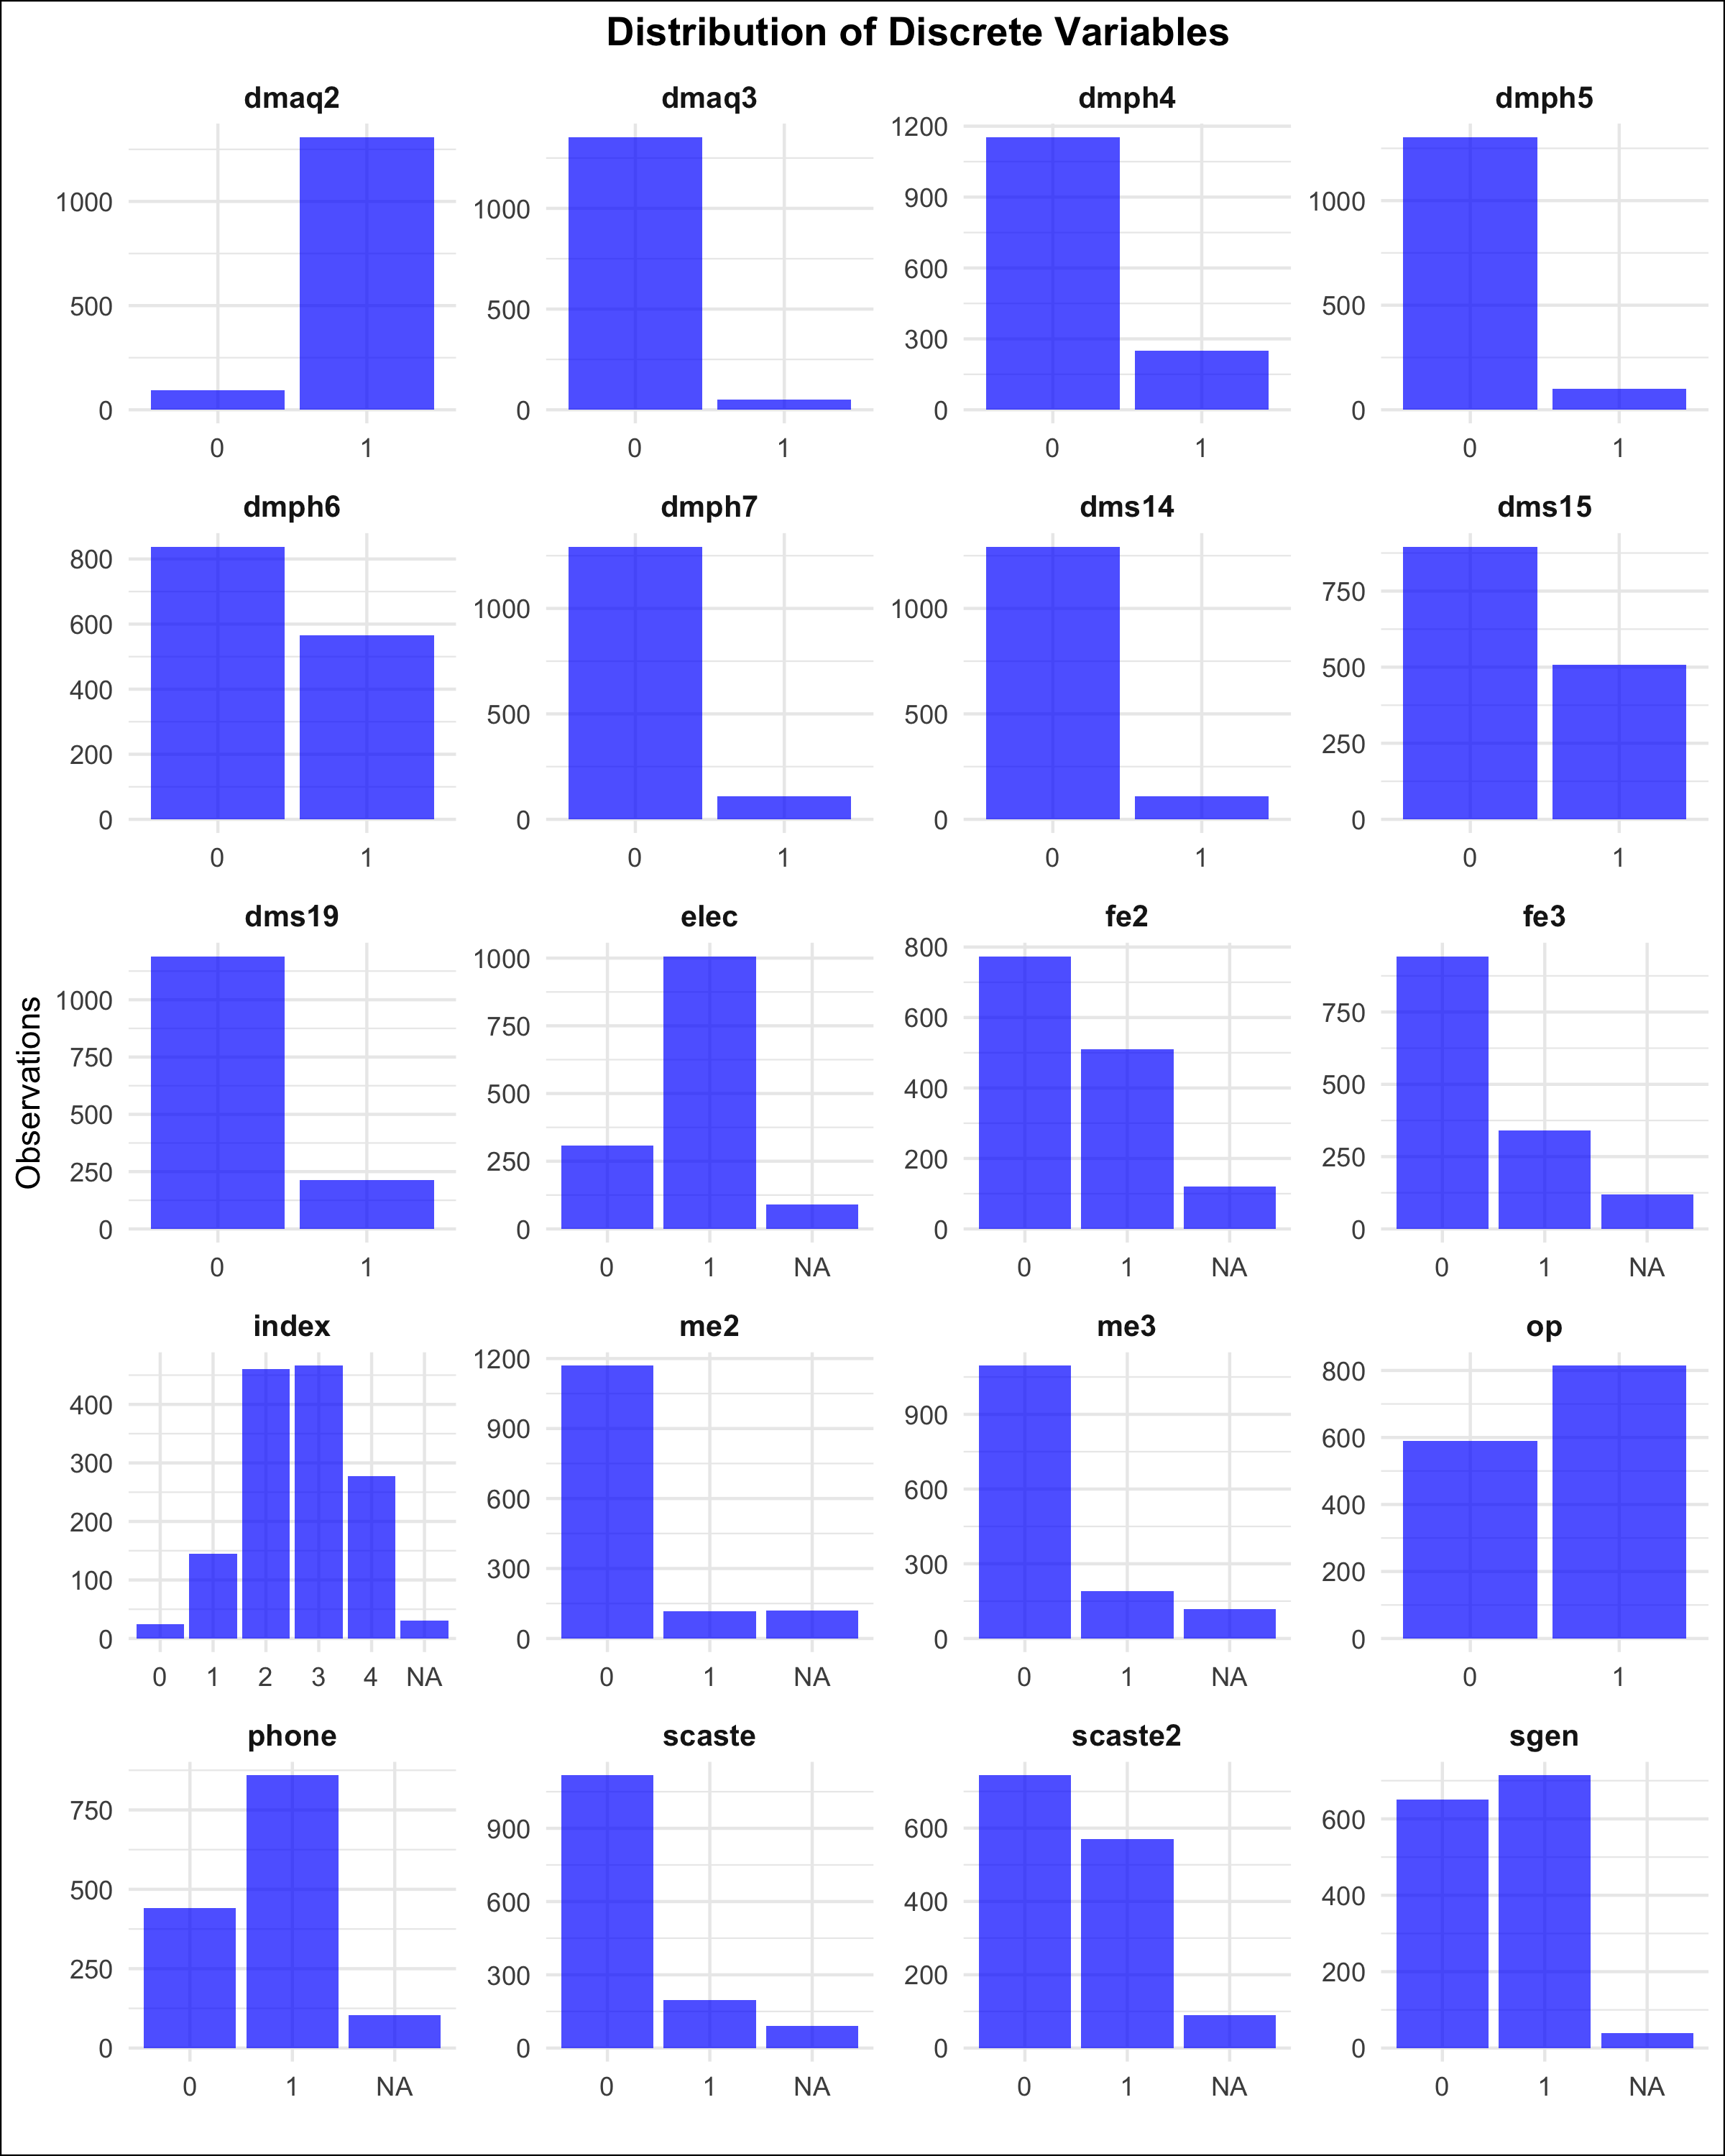
\includegraphics[width=1\textwidth]{OUTPUT/MEDIA/score_bar.png}  % Remplacez par le chemin de votre image
    \label{fig:bar}
\end{figure}
\begin{figure}[p]  % 'p' place la figure sur une page dédiée
    \centering
    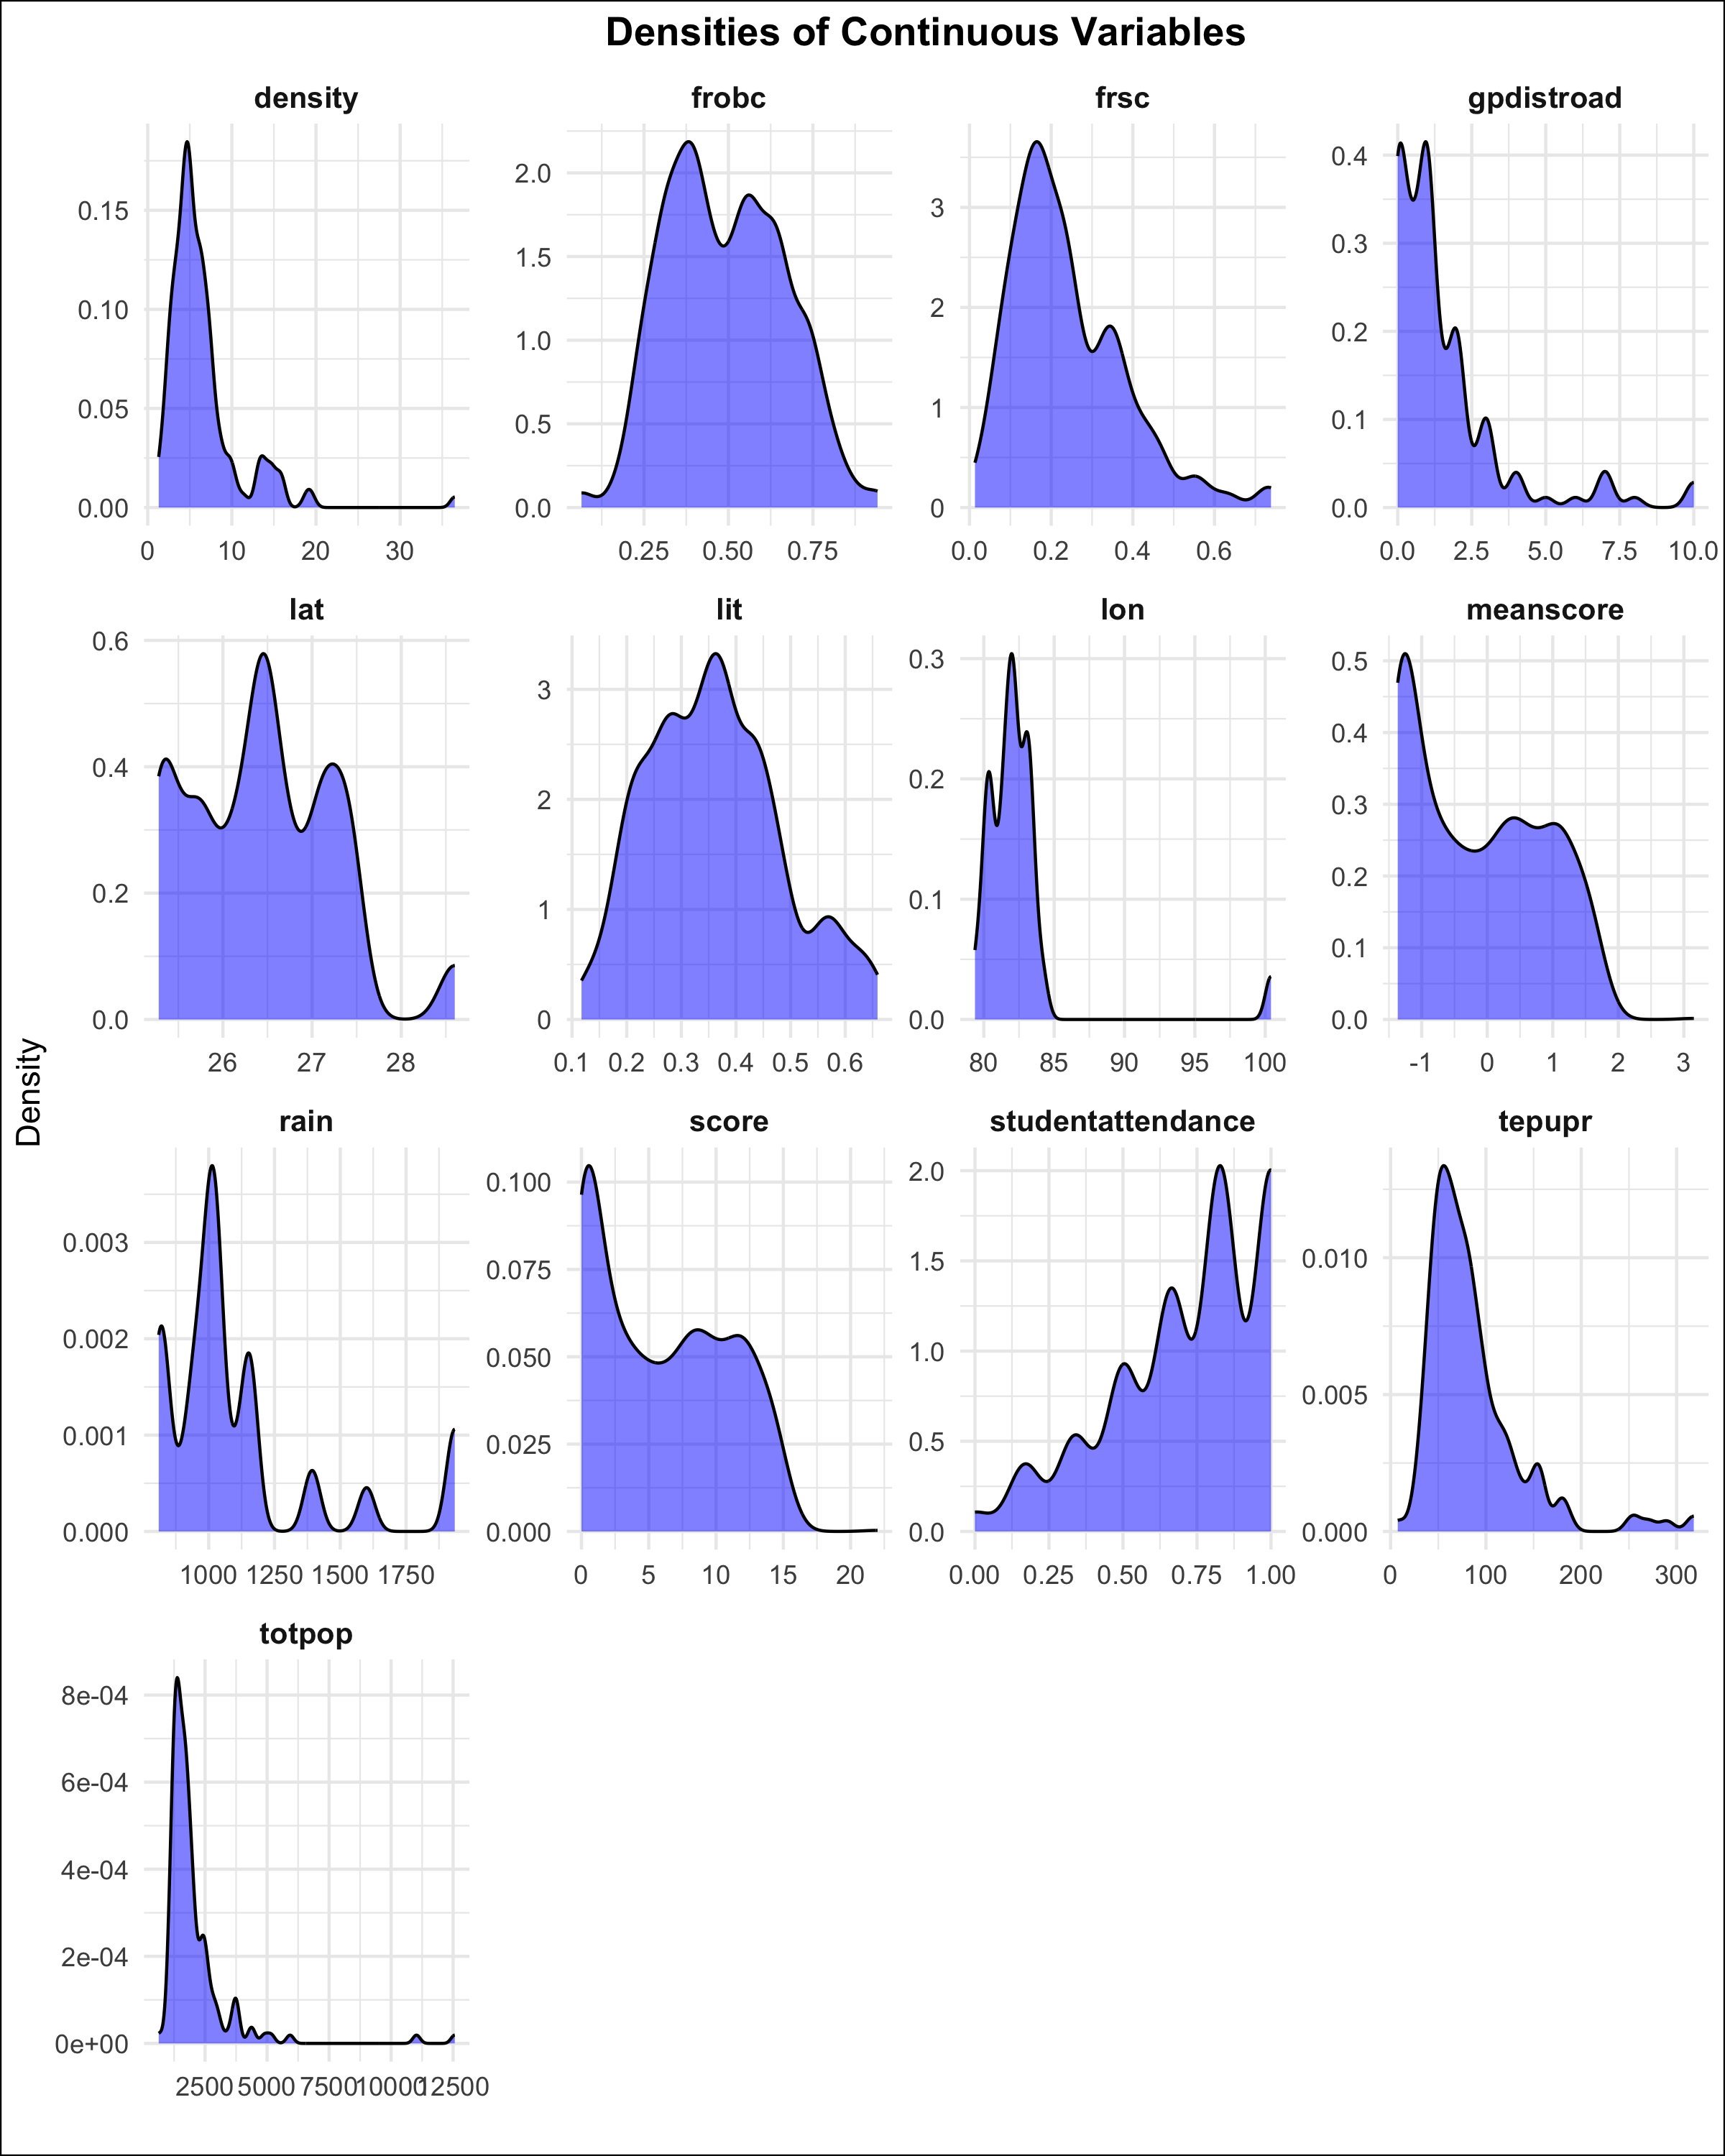
\includegraphics[width=1\textwidth]{OUTPUT/MEDIA/score_density.png}  % Remplacez par le chemin de votre image
    \label{fig:density}
\end{figure}
\begin{figure}[p]  % 'p' place la figure sur une page dédiée
  \centering
  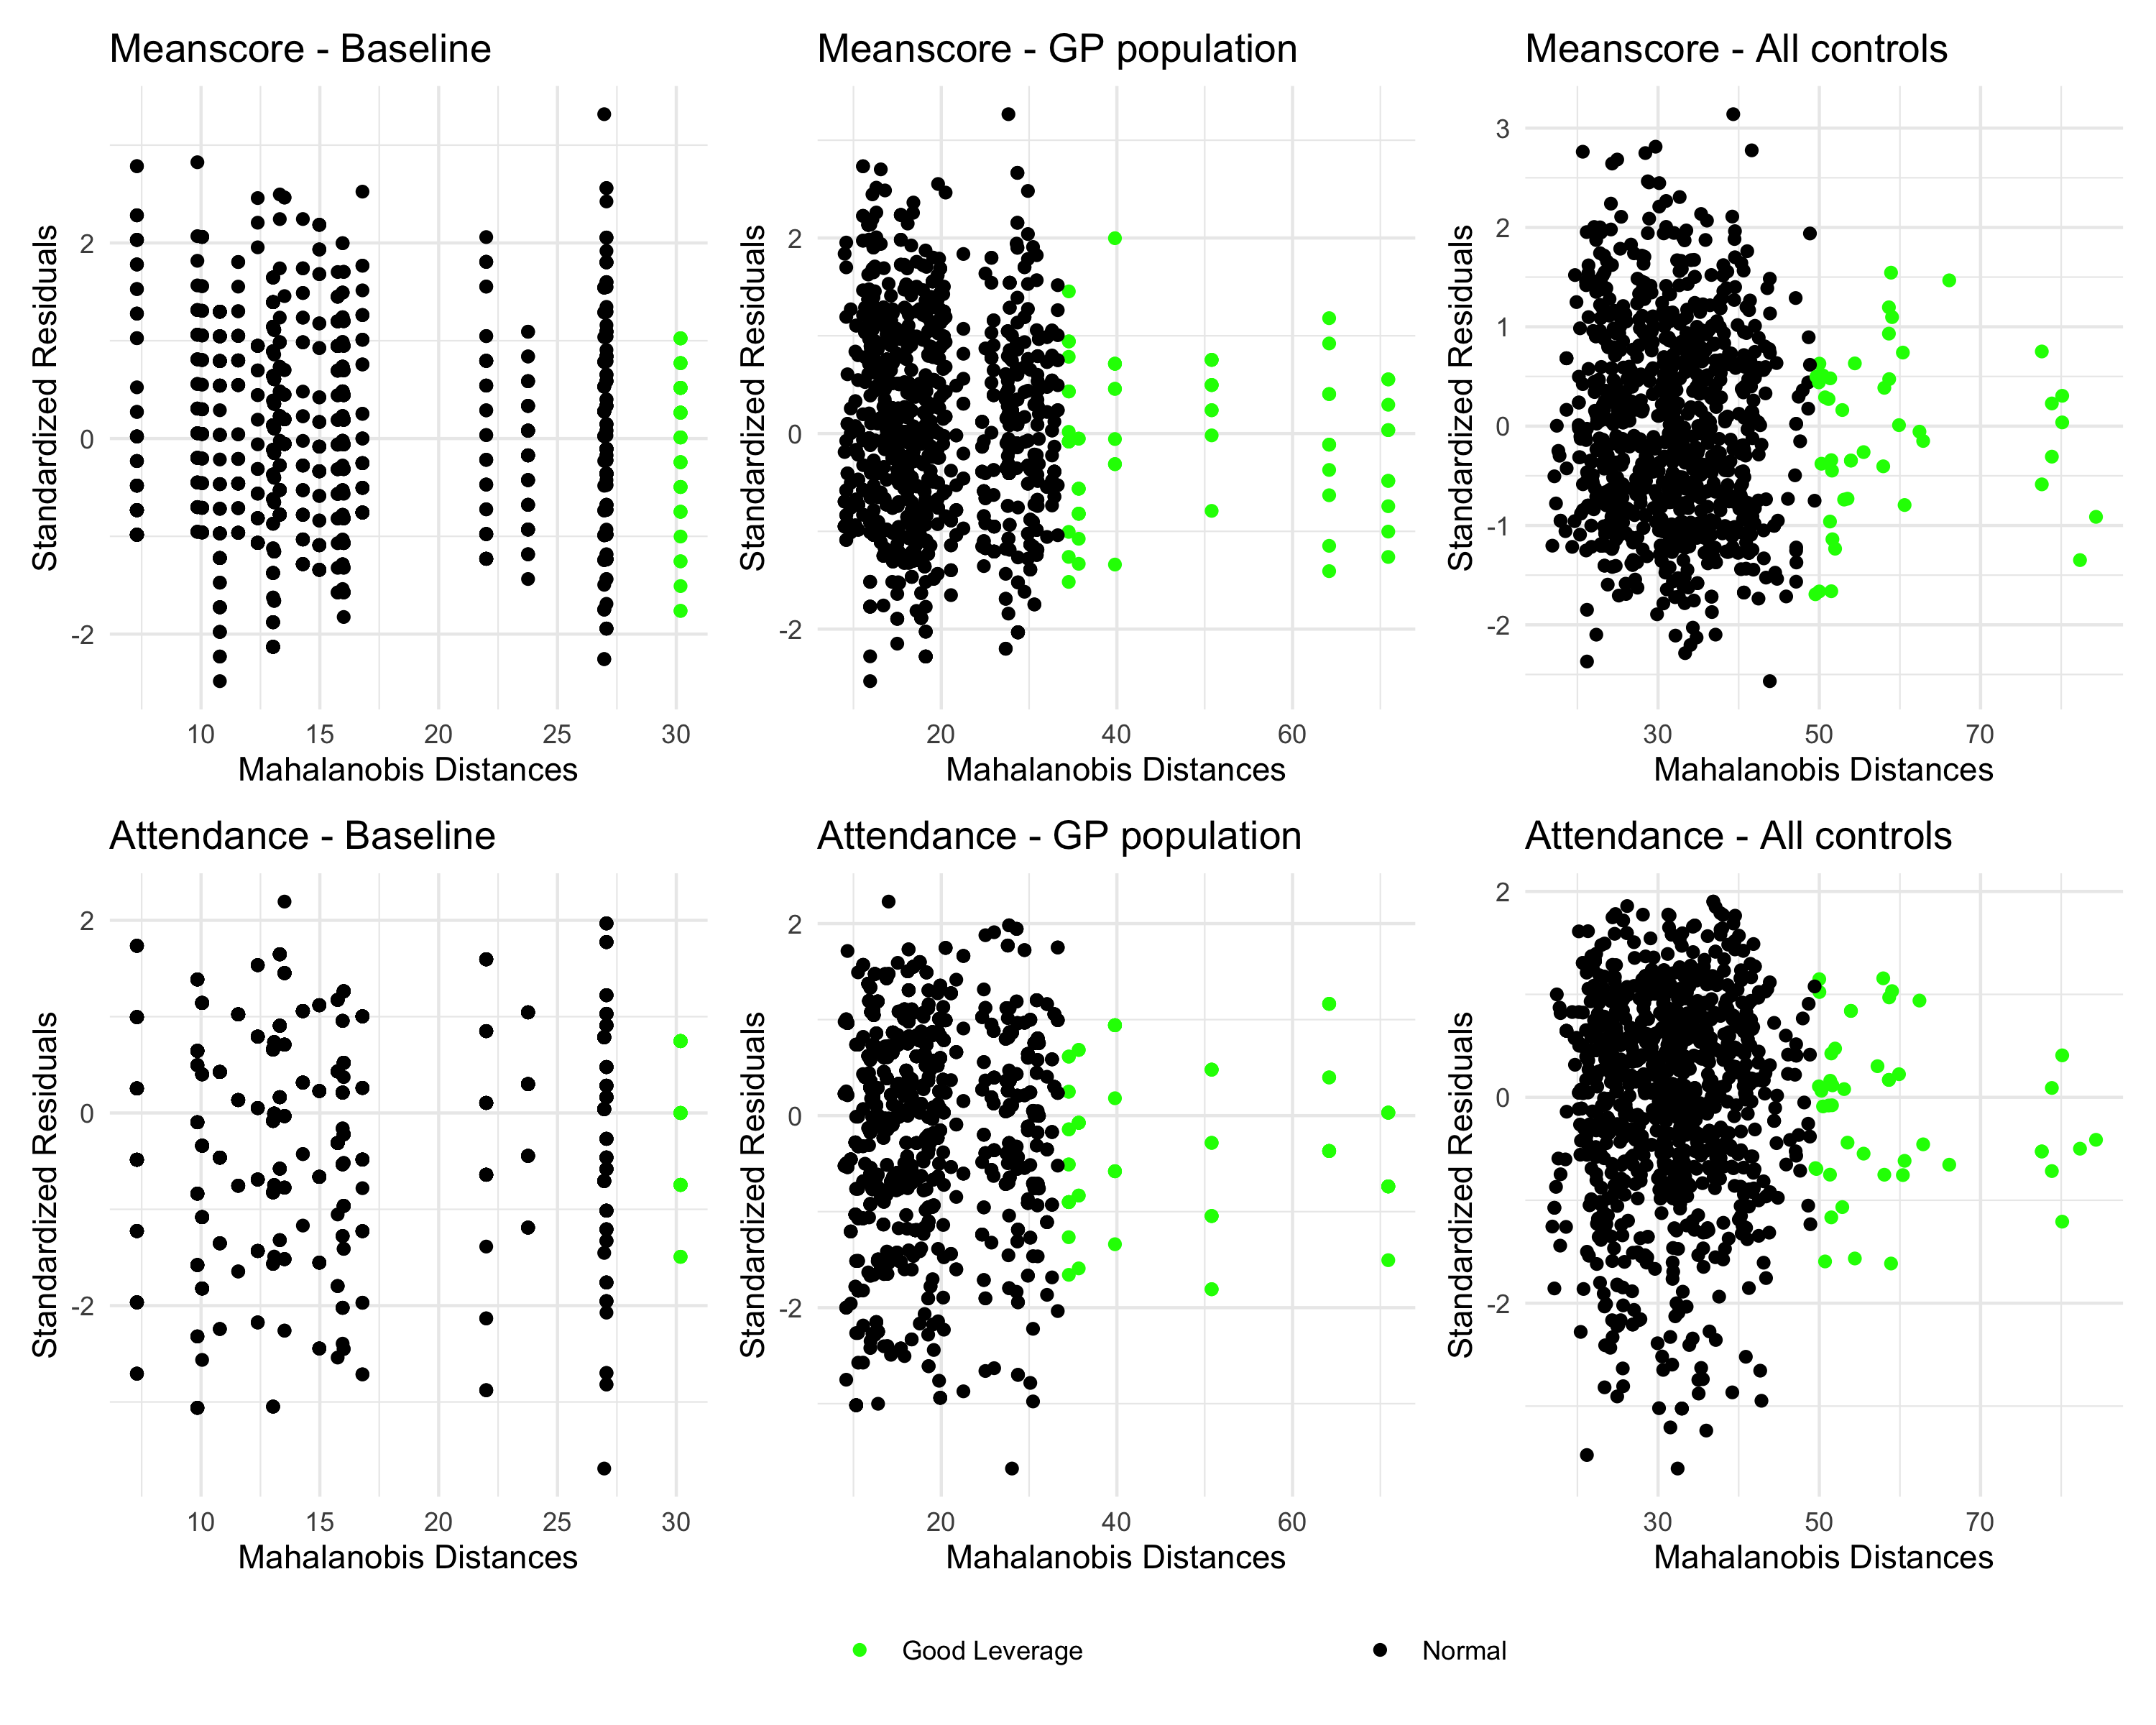
\includegraphics[width=1\textwidth]{OUTPUT/MEDIA/manhalobis.png}  % Remplacez par le chemin de votre image
  \label{fig:manhalobis}
\end{figure}

\begin{figure}[p]
  \centering
  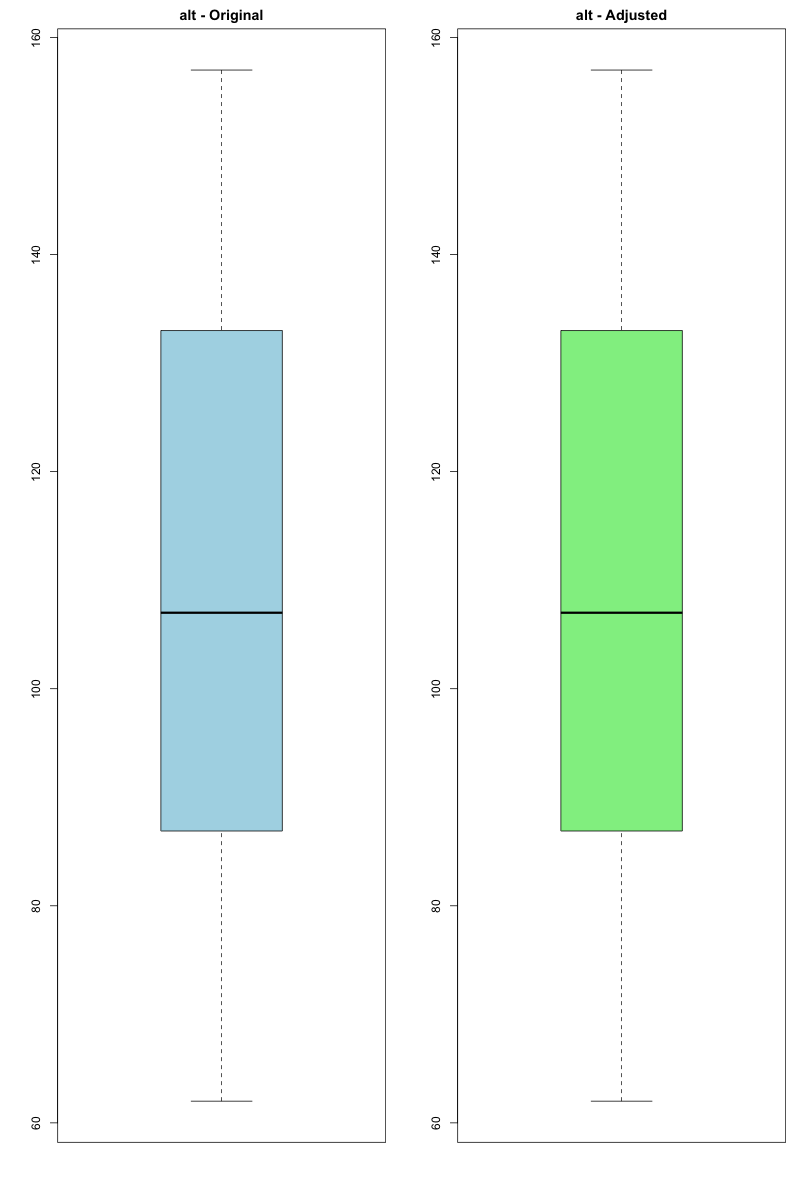
\includegraphics[width=0.299\textwidth]{OUTPUT/BOXPLOTS/alt.png}
  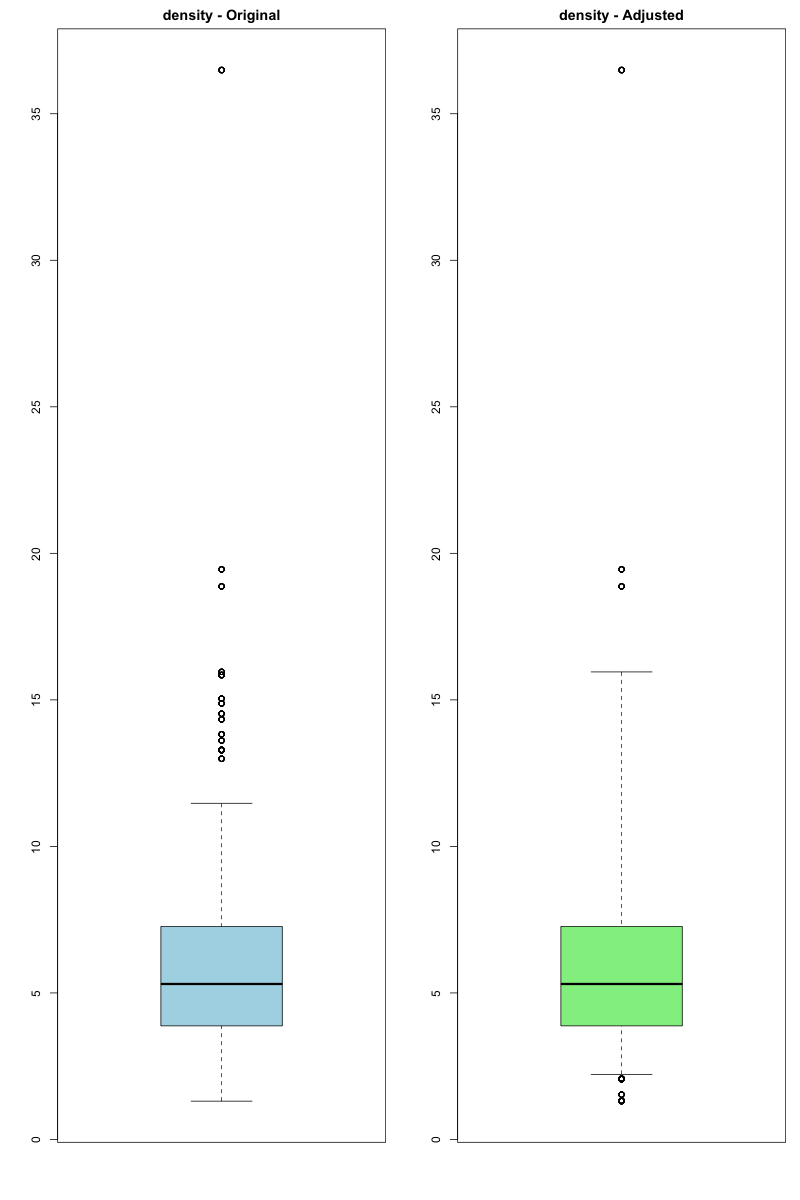
\includegraphics[width=0.299\textwidth]{OUTPUT/BOXPLOTS/density.png}
  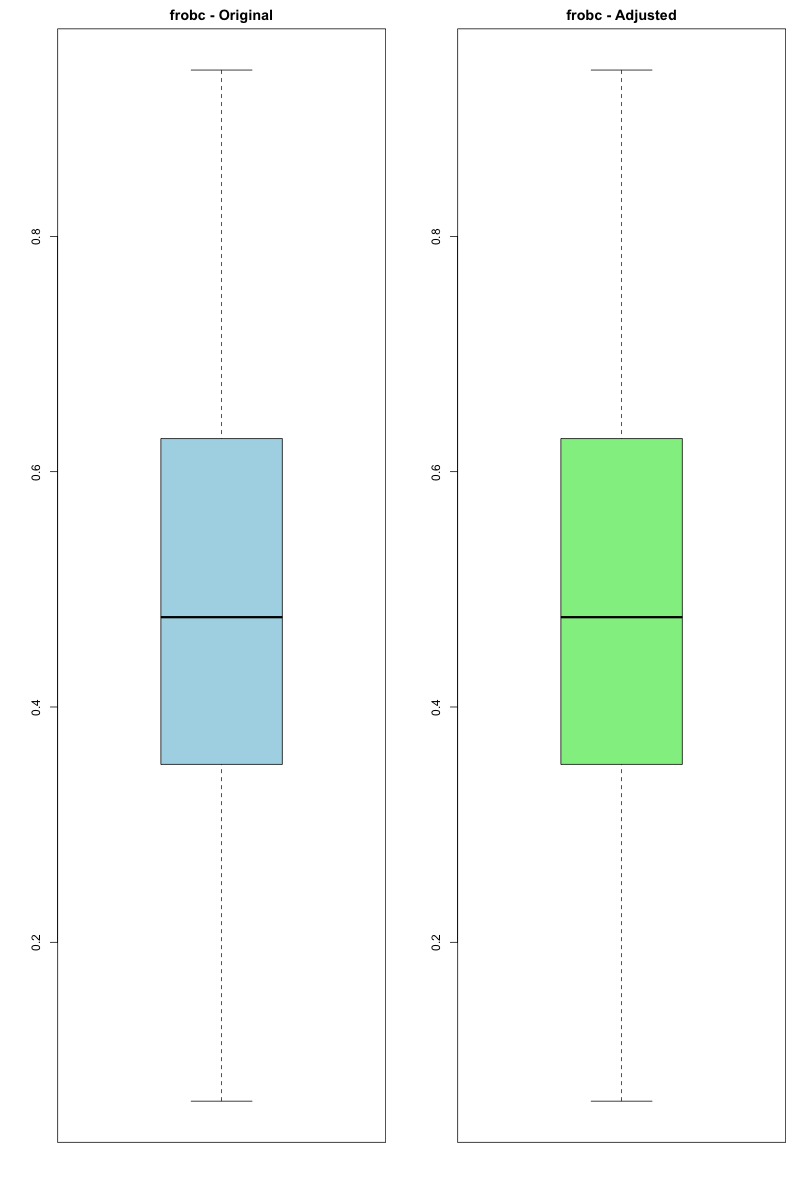
\includegraphics[width=0.299\textwidth]{OUTPUT/BOXPLOTS/frobc.png}
  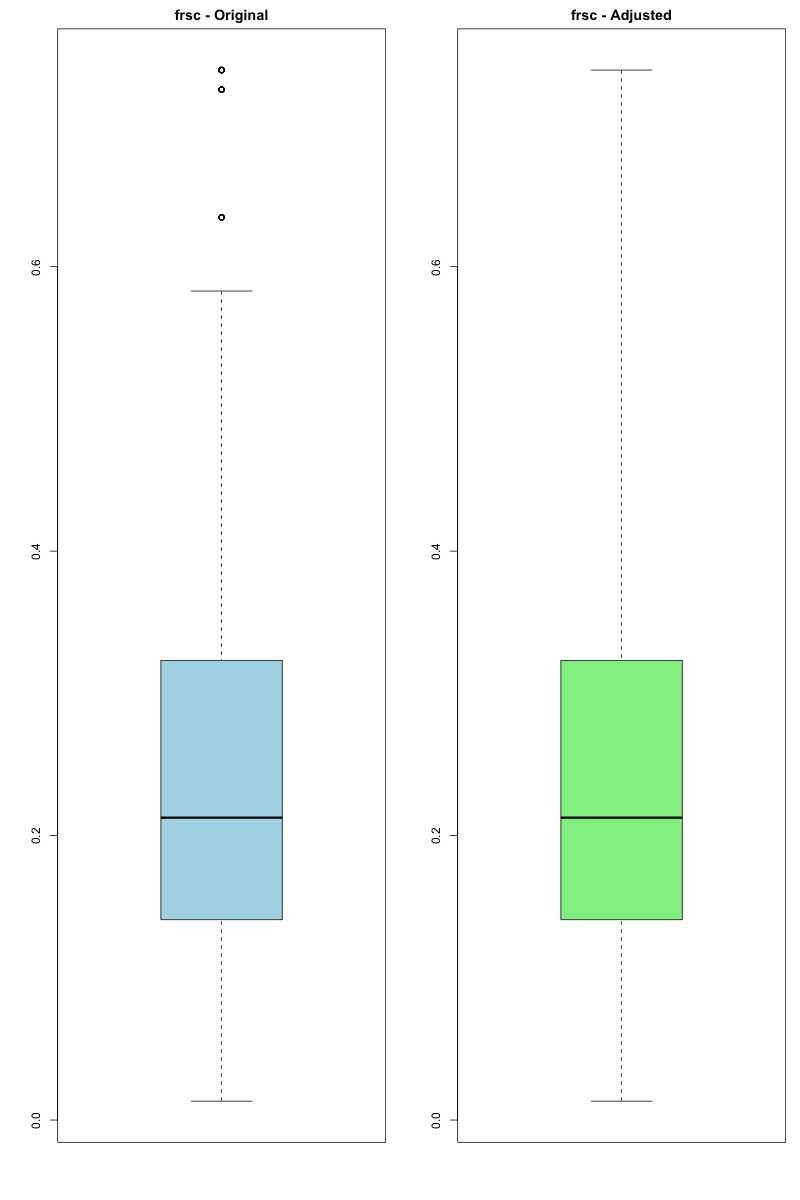
\includegraphics[width=0.299\textwidth]{OUTPUT/BOXPLOTS/frsc.png}
  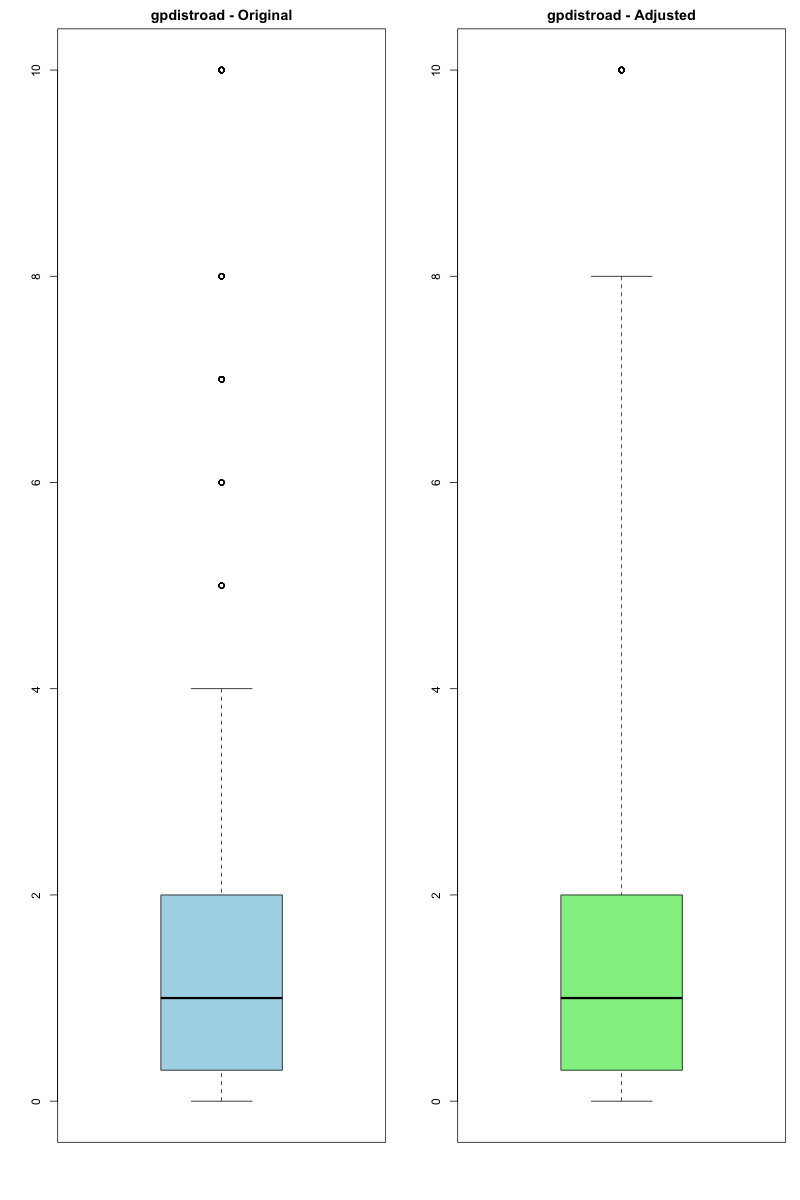
\includegraphics[width=0.299\textwidth]{OUTPUT/BOXPLOTS/gpdistroad.png}
  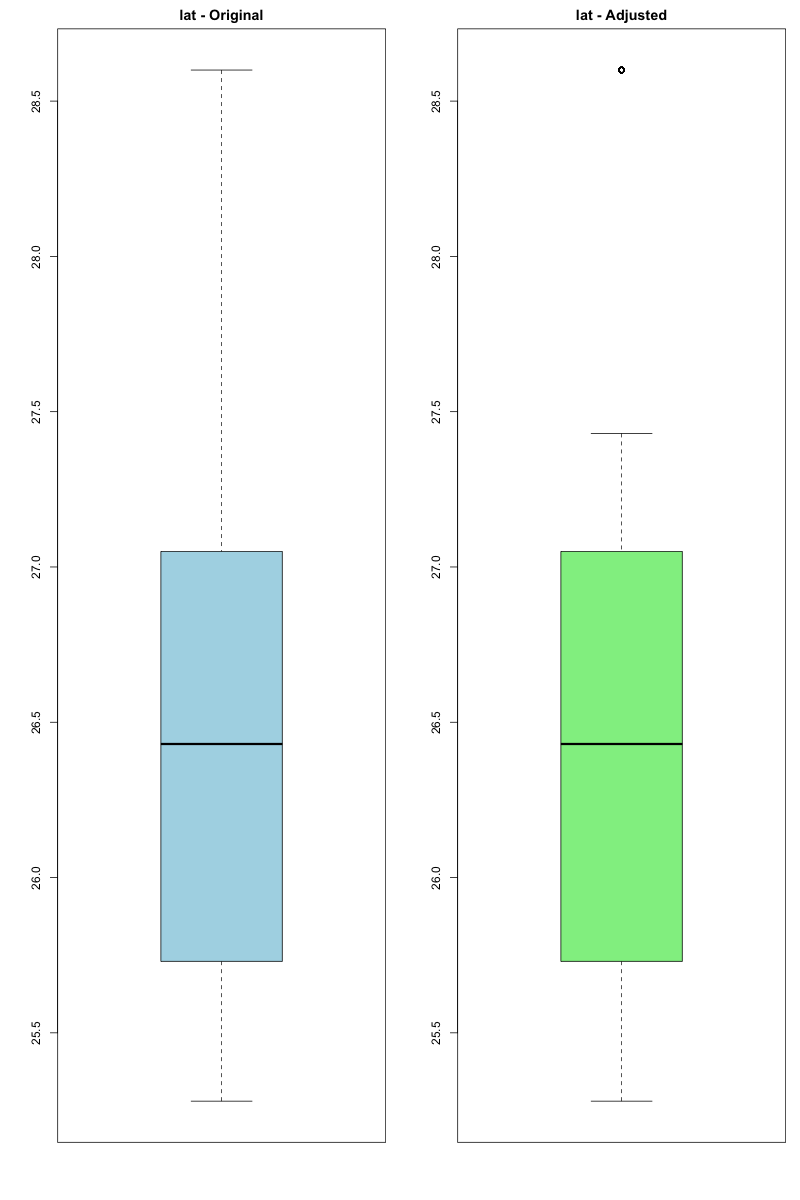
\includegraphics[width=0.299\textwidth]{OUTPUT/BOXPLOTS/lat.png}
  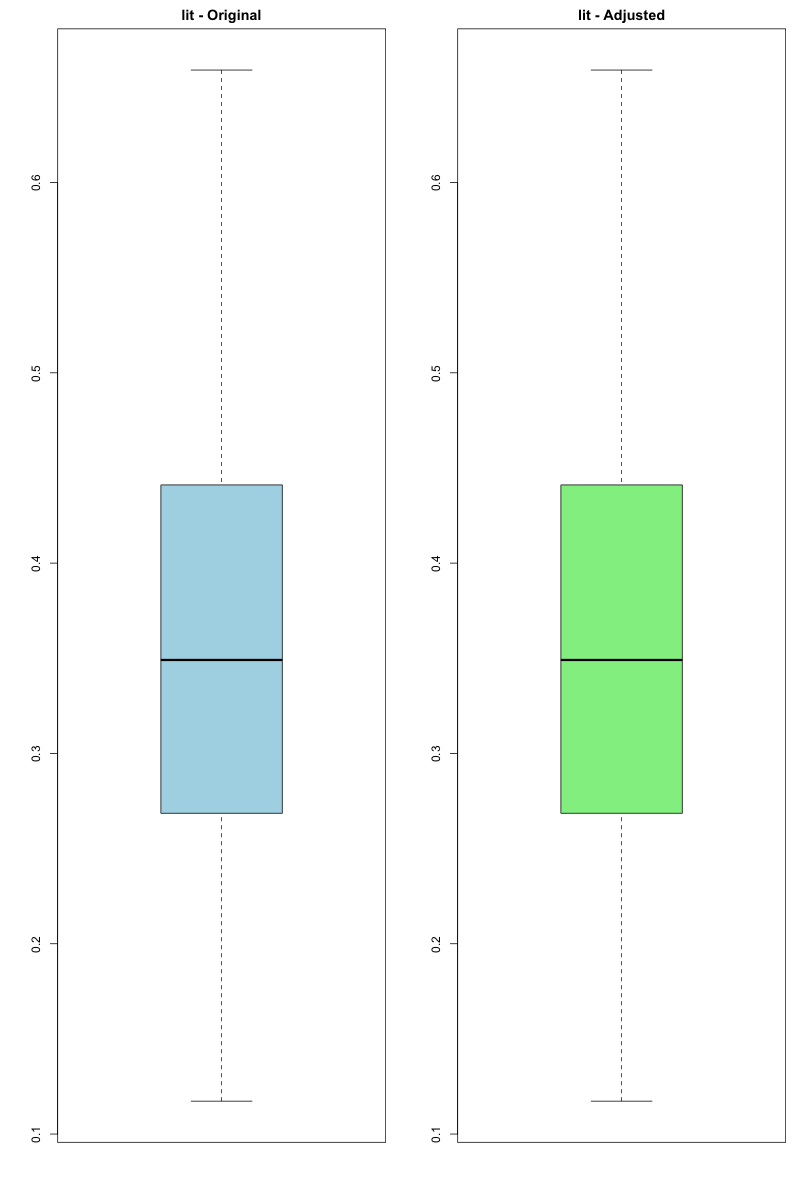
\includegraphics[width=0.299\textwidth]{OUTPUT/BOXPLOTS/lit.png}
  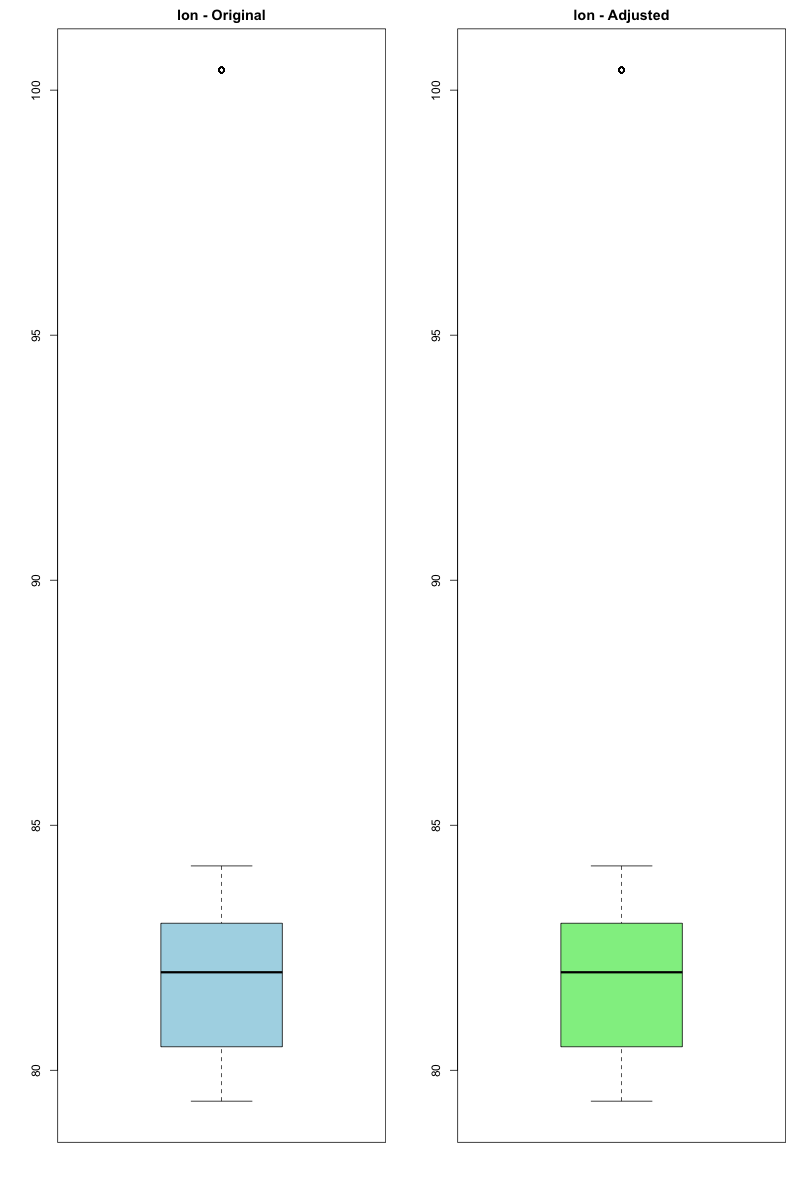
\includegraphics[width=0.299\textwidth]{OUTPUT/BOXPLOTS/lon.png}
  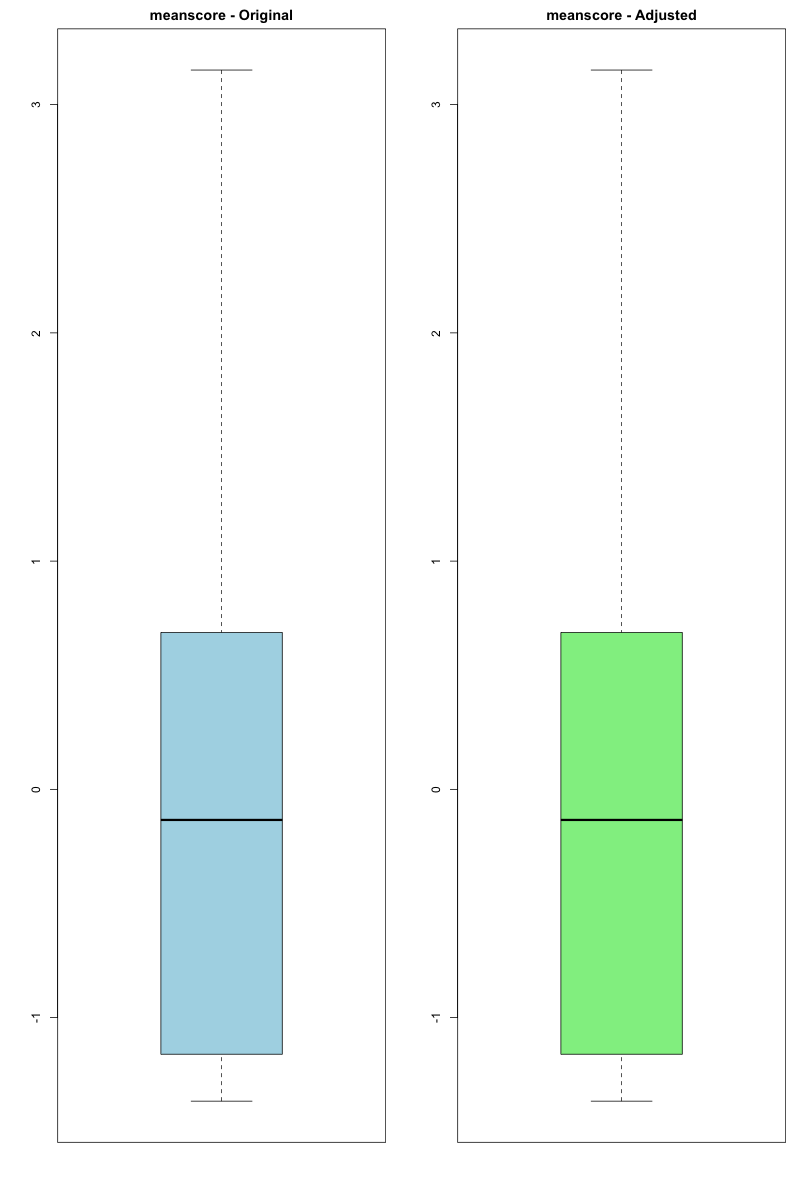
\includegraphics[width=0.299\textwidth]{OUTPUT/BOXPLOTS/meanscore.png}
  \label{fig:boxplots1}
\end{figure}
\begin{figure}[p]
  \centering
  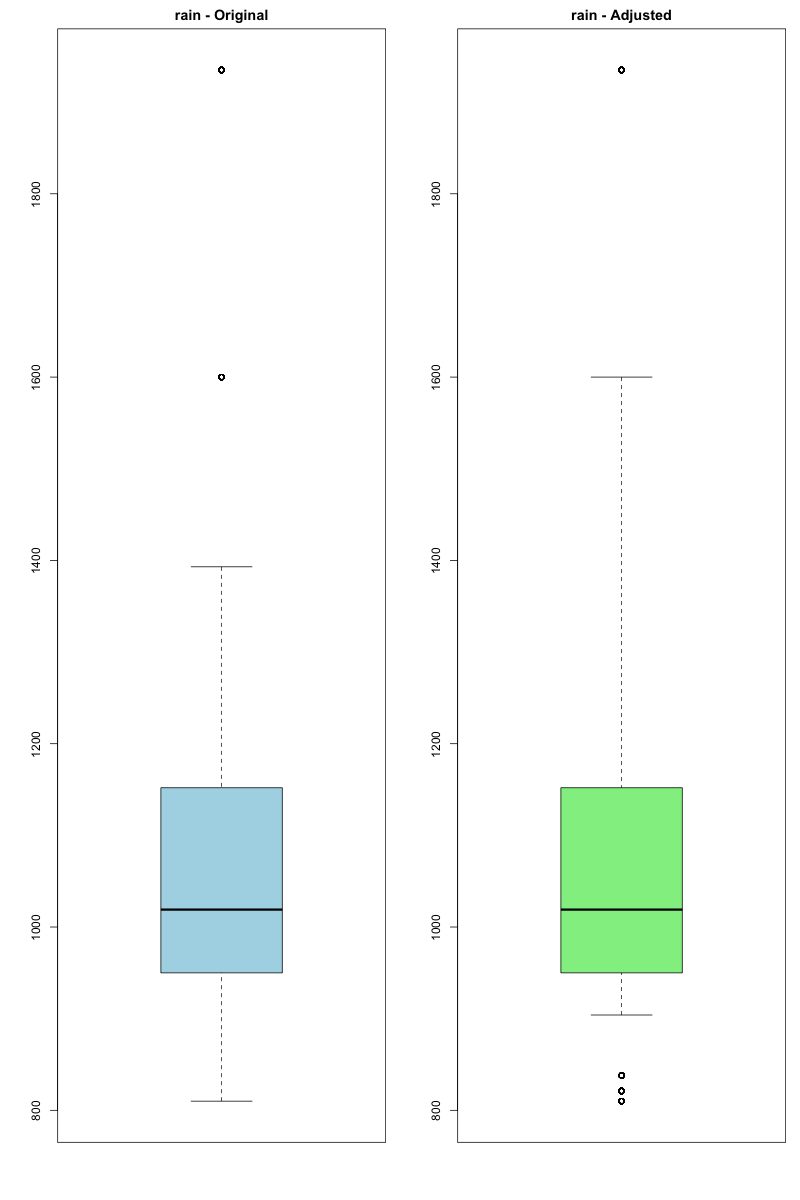
\includegraphics[width=0.299\textwidth]{OUTPUT/BOXPLOTS/rain.png}
  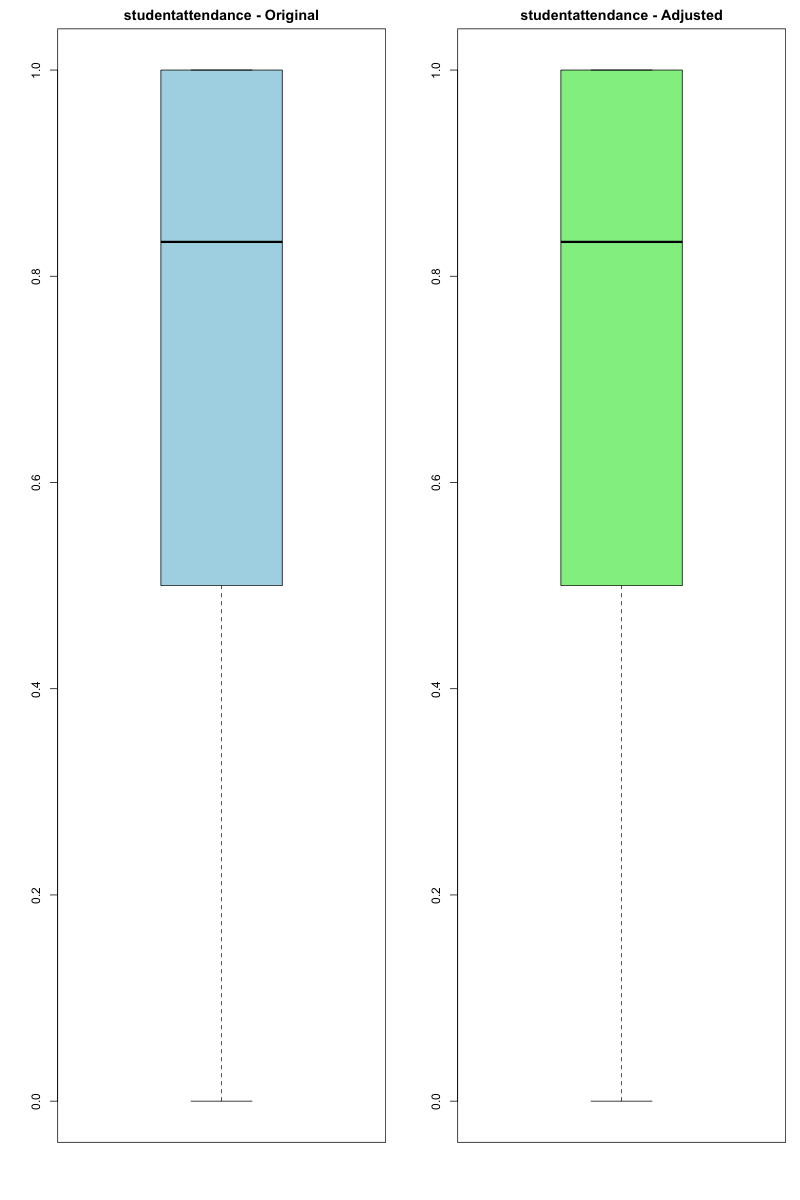
\includegraphics[width=0.299\textwidth]{OUTPUT/BOXPLOTS/studentattendance.png}
  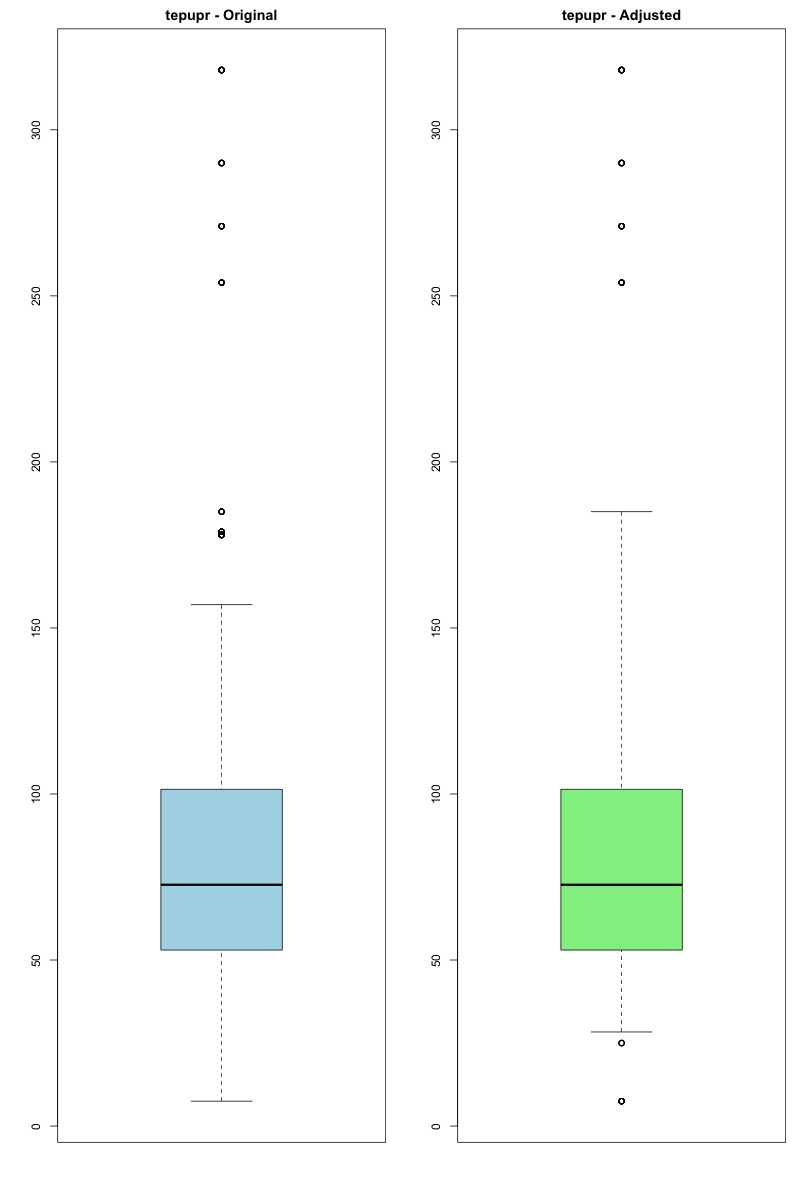
\includegraphics[width=0.299\textwidth]{OUTPUT/BOXPLOTS/tepupr.png}
  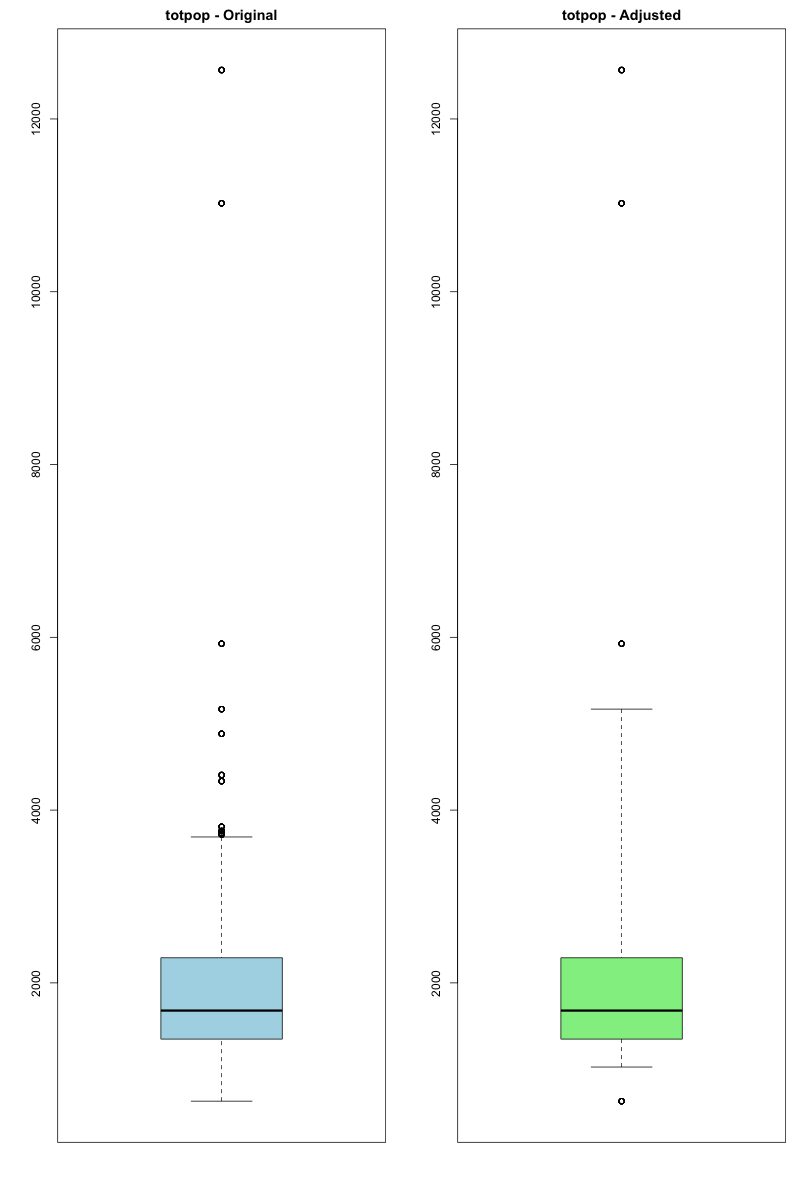
\includegraphics[width=0.299\textwidth]{OUTPUT/BOXPLOTS/totpop.png}

  \label{fig:boxplots2}
\end{figure}


\end{document}